%%「論文」,「レター」,「レター(C分冊)」,「技術研究報告」などのテンプレート
%% v3.4 [2023/09/12]
%% 1. 「論文」
% \documentclass[paper]{ieicej}
\documentclass[technicalreport]{ieicej}

% \documentclass[invited]{ieicej}% 招待論文
%\documentclass[survey]{ieicej}% サーベイ論文
%\documentclass[comment]{ieicej}% 解説論文
\usepackage[dvipdfmx]{graphicx,xcolor}
%%\usepackage[dvips]{graphicx}
\usepackage[fleqn]{amsmath}
%\usepackage{amsthm}
\usepackage{newtxtext}% 英数字フォントの設定を変更しないでください
\usepackage[varg]{newtxmath}% % 英数字フォントの設定を変更しないでください
%\usepackage{amssymb}
%\usepackage{bm}
\usepackage{listings,jvlisting} %日本語のコメントアウトをする場合jvlisting(もしくはjlisting)が必要
%ここからソースコードの表示に関する設定
\lstset{
  basicstyle={\ttfamily},
  identifierstyle={\small},
  commentstyle={\smallitshape},
  keywordstyle={\small\bfseries},
  ndkeywordstyle={\small},
  stringstyle={\small\ttfamily},
  frame={tb},
  breaklines=true,
  columns=[l]{fullflexible},
  numbers=left,
  xrightmargin=0zw,
  xleftmargin=3zw,
  numberstyle={\scriptsize},
  stepnumber=1,
  numbersep=1zw,
  lineskip=-0.5ex,
  % extendedchars=false, % ★ 日本語の縦書き化を防止
}
\renewcommand{\lstlistingname}{プログラム}% ソースコードのキャプションの名称

\setcounter{page}{1}

\field{A}
\jtitle{状態遷移図ベースのコード生成とログ可視化機能を備えたセンサネットワーク実機検証基盤の開発}
\etitle{}
\authorlist{%
 \authorentry[24w6047a@shinshu-u.ac.jp]{辻村篤志}{Atsushi Tsujimura}{信州大学}\MembershipNumber{}
 \authorentry{小林侑生}{Yu Kobayashi}{信州大学}\MembershipNumber{}
 \authorentry{不破泰}{Yasushi Fuwa}{信州大学}\MembershipNumber{}
 \authorentry{アサノデービッド}{David Asano}{信州大学}\MembershipNumber{}
 %\authorentry{和文著者名}{英文著者名}{所属ラベル}\MembershipNumber{}
 %\authorentry[メールアドレス]{和文著者名}{英文著者名}{所属ラベル}\MembershipNumber{}
 %\authorentry{和文著者名}{英文著者名}{所属ラベル}[現在の所属ラベル]\MembershipNumber{}
}
\affiliate[Nagano]{信州大学 〒380-0928 長野県長野市若里4-17-1}
 {Shinshu University, 4--17--1 Wakasato, Nagano-shi, 
  Nagano 380--8553 Japan}
%\affiliate[所属ラベル]{和文所属}{英文所属}
%\paffiliate\[]{}
%\paffiliate[現在の所属ラベル]{和文所属}
\jalcdoi{???????????}% ← このままにしておいてください

\begin{document}
\begin{abstract}
%和文あらまし 500字以内
センサネットワークの開発は幅広い専門知識と多大な工数を要する。先行研究では、センサネットワークの動作を表す状態遷移図からコードを生成し、汎用ハード上で動作する環境が構築されてきた。本研究ではその環境を拡張し、その上で実用的な無線通信プロトコルを実装・検証した。その過程で汎用ハード上でのプロトコルの動作が確認しづらいことを課題として認識し、デバッグ用ログ出力とそれを可視化・ステップ実行できる環境を開発しデバッグ効率の向上を図った。
\end{abstract}
\begin{keyword}
%和文キーワード 4〜5語
無線センサーネットワーク、無線通信プロトコル、状態遷移図、コード生成、ログ可視化
\end{keyword}

\begin{eabstract}
%英文アブストラクト 100 words
The development of sensor networks requires extensive expertise and significant effort. Previous research has generated code from state transition diagrams representing the behavior of sensor networks, establishing an environment that operates on general-purpose hardware. This study expands that environment and implements and verifies practical wireless communication protocols. During this process, we recognized the difficulty in confirming the operation of protocols on general-purpose hardware as a challenge and developed an environment for debugging log output and visualizing and step-executing it to improve debugging efficiency.
\end{eabstract}

\begin{ekeyword}
%英文キーワード
wireless sensor networks, wireless communication protocols, state transition diagrams, code generation, log visualization
\end{ekeyword}
\maketitle

% _/_/_/_/_/_/_/_/_/_/_/_/_/_/_/_/_/_/_ 1章 /_/_/_/_/_/_/_/_/_/_/_/_/_/_/_/_/_/_/_/_/_/_/_/_/_/_/_/_/_/_/
\section{はじめに}
\subsection{背景}
近年、無線センサネットワーク(Wireless Sensor Network:WSN)は、環境モニタリングやスマートシティ、インフラ監視、農業、ヘルスケアなど、さまざまな分野での応用が期待されている。実際、WSNを含むIoTデバイスの数は2020年時点で約130億台に達し、年率20%で増加しており、2025年には300億台弱に到達すると予測されている\cite{jst2022}. また、MDPIの報告によれば、WSNノードの数は2012年の約4.5億台から2022年には約20億台へと拡大しており\cite{mdpi2021}、その研究および実用の両面での発展が顕著である。  
しかし、これらのシステムを構築するためには、複雑な通信プロトコル設計やデータ処理アルゴリズムの実装が求められ、開発者には高度な専門知識と多大な工数が必要となる。さらに、無線通信環境の構築やマイコン設定など導入時のハードルも高く、これらの研究や開発の多くはシミュレーション環境やエミュレータ上での検証にとどまることが多い。
\vskip\baselineskip

\subsection{従来研究}
従来研究では、無線通信プロトコルの状態遷移図から自動生成したプログラムを汎用ハード上で動作させ、プロトコルを実機で実装・検証できる環境が構築されていた(旭ら\cite[asahi])。このシステムにより基本的な通信プロトコルの動作検証が可能となったが、デバッグ方法はシリアルコンソールへのログ出力に依存しており、通信処理が高速に進むため逐次的な状態遷移を追跡することが難しかった。その結果、複雑な動作を含むプロトコルに対しては、異常動作の原因を把握しづらく、開発効率や教育的利用の観点では十分でない点が課題として残されていた。

\vskip\baselineskip
\subsection{目的}
本研究の目的は、従来研究で課題となっていたデバッグ効率の低さを改善し、実機でのプロトコル検証をより効果的に行える環境を実現することである。そのために、状態遷移図から生成したコードの動作をログとして出力し、それを可視化・ステップ実行できる仕組みを開発した。これにより、プロトコルの動作を逐次的に把握でき、異常動作の原因究明を容易にするとともに、教育や応用実証に適した支援環境を提供することを目指す。
\vskip\baselineskip




% _/_/_/_/_/_/_/_/_/_/_/_/_/_/_/_/_/_/_ 2章 /_/_/_/_/_/_/_/_/_/_/_/_/_/_/_/_/_/_/_/_/_/_/_/_/_/_/_/_/_/_/
\section{提案システム}
\subsection{システム構成}
本研究で開発したシステムの全体構成を図\ref{fig:system-composition}に示す。本システムは、状態遷移図を入力としてC++プログラムを自動生成し、PlatformIO上でビルドを行い、汎用ハードウェア上で実行することでセンサネットワークのプロトコルの動作検証を可能とする。さらに、通信動作の状態遷移や変数値変化の過程をログとして記録し、ブラウザ上で状態遷移の可視化およびステップ実行を行える環境を備えている。これにより、プロトコル設計から実機検証、デバッグまでを一貫して支援することが可能となる。
\vskip\baselineskip
\begin{figure}[h]
  \centering
  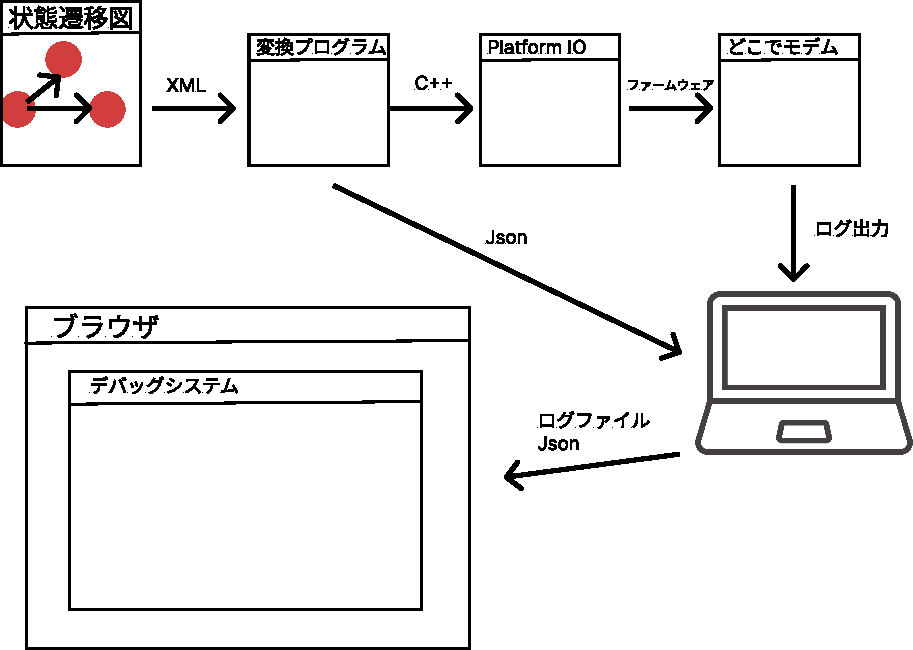
\includegraphics[width=80mm]{./images/system-composition.pdf}
  \caption{提案システムの全体構成}
  \ecaption{Block diagram of the proposed system.}
  \label{fig:system-composition}
\end{figure}


\subsection{ファームウェア生成部}
ファームウェア生成部では,無線通信プロトコルの動作をAstah Professional上の状態遷移図として設計し,XML形式で出力する。次に,変換プログラム(Python)を用いて状態遷移図のXMLをC++プログラムへ変換し,PlatformIO環境でビルドすることでファームウェアを生成する。このファームウェアは2.3節で述べる汎用ハードウェア上で実行される。

先行研究(小林ら\cite{kobayashi2023})では,状態遷移図の各要素(通信状態・遷移・初期値設定・処理内容など)をXMLファイルから抽出し,C++の`switch-case`構造に変換するアルゴリズムが実装されている。本研究におけるファームウェア生成部は,この変換処理を利用しており,状態遷移図で設計されたプロトコル仕様を汎用ハードウェア上で動作するプログラムとして自動生成するものである。

図\ref{fig:state-machine}に状態遷移図の例を,プログラム\ref{converted-code}に変換後のC++プログラムを示す。状態遷移図で定義された「待機(LISTEN)」「受信(RECEIVE)」「送信(TRANSMIT)」の各状態と遷移関係が,`switch-case`構造によって対応づけられており,設計段階の論理構造がソースコードとして正しく反映されていることが確認できる。

\vskip\baselineskip
\begin{figure}[tb]
  \centering
  \includegraphics[width=60mm]{./images/state-machine-image.png}
  \caption{状態遷移図の例}
  \ecaption{State transition diagram.}
  \label{fig:state-machine}
\end{figure}

\begin{figure}
\begin{lstlisting}[caption={変換されたC++プログラム}, label=converted-code]
typedef enum { LISTEN, RECEIVE, TRANSMIT } NodeState;

void protocol_main() {
  switch (state) {
    case LISTEN:   updateState(RECEIVE);   break;
    case RECEIVE:  updateState(TRANSMIT);  break;
    case TRANSMIT: updateState(LISTEN);    break;
  }
}
\end{lstlisting}
\end{figure}
\vskip\baselineskip




\subsection{実行環境(ハードウェア)}
本システムにおける実行環境を図\ref{fig:devices}に示す。本研究では,SAMD21マイコンと無線通信モジュールを一体化した無線通信デバイス(株式会社サーキットデザイン製どこでモデム)を使用した。この無線通信モジュールは429MHz帯で動作する汎用的なものであり,技術基準適合証明(技適)を取得しているため,実際に電波飛ばしながら通信プロトコルの検証を行うことができる。また,429MHz帯は中山間地域において回折性能に優れており,低消費電力で長距離通信が可能なLPWA(Low Power Wide Area)通信に適している。この特性を活かすことで,登山者見守りシステムなどへの応用も期待できる。さらに,本デバイスはマイコンと通信モジュールが一体化しているため,外部配線や追加ハードウェアを必要とせず,開発や実験環境の構築を容易に行うことが可能である。加えて,GPSモジュールを併用することで,位置情報の取得および1PPS信号による高精度な時刻同期を実現し,複数ノード間での無線通信プロトコルの正確な動作検証を可能としている。
\vskip\baselineskip
\begin{figure}[tb]
  \centering
  \includegraphics[width=60mm]{./images/devices.jpg}
  \caption{どこでモデム(左)とGPSモジュール(右)}
  \ecaption{Block diagram of the proposed system.}
  \label{fig:devices}
\end{figure}


\subsection{デバッグシステム部}
本節では,通信プロトコルの動作を可視化し,逐次的なデバッグを可能とするデバッグシステムについて述べる。本システムは,通信プロトコルの状態遷移および変数変化をログとして記録し,ブラウザ上でそのログを可視化・ステップ実行できる環境を提供する。これにより,通信動作の流れを直感的に把握でき,異常動作の原因究明や設計検証を効率化することが可能となる。
\vskip\baselineskip

\subsubsection{UI構成}
図\ref{fig:viewer-ui}に可視化画面の構成を示す。画面上部にログファイル(テキスト)および状態遷移図ファイル(JSON)のアップロード領域を配置し,中央にステップ実行用のボタン群(次,前,最初に戻る)とスライダを設ける。下部は「変数追跡」「ログ表示」「状態遷移図描画」の3領域で構成し,処理の流れと内部状態を統合的に把握できる設計とした。
% UIの画像
\begin{figure}[b]
  \centering
  \includegraphics[width=80mm]{./images/viewer_ui.png}
  \caption{ログ可視化・ステップ実行環境のUI}
  \ecaption{User interface of the log visualization and step execution environment.}
  \label{fig:viewer-ui}
\end{figure}
\vskip\baselineskip

\subsubsection{ログ出力形式}
状態遷移や変数を逐次ログとして出力し、それを可視化・解析するために,ログの出力形式を統一した。具体的には,状態遷移は
\begin{verbatim}
STATE:LISTEN
STATE:RECEIVE
\end{verbatim}
のように1行1状態で出力し,変数は
\begin{verbatim}
[VAR:current_slot=3]
[VAR:has_own_slot=true]
\end{verbatim}
のように \verb|[VAR:<name>=<value>]| 形式で出力する。値は数値・文字列の双方を許容し,可視化側で時間順に解析する。単純で曖昧さの少ない表記とすることで,正規表現に基づく軽量なパーサで高速に処理できる。

さらに,ログ出力の形式にばらつきが生じないよう,C++のマクロを用いてログ出力関数を定義している。このマクロは,変数名と値を自動的に取得して \verb|[VAR:<name>=<value>]| 形式で出力するため,開発者は変数名を明示する必要がない。例えば,ユーザは \verb|PRINT_VAR_LOG(変数)| のように記述するだけで統一フォーマットのログを生成できる。この仕組みにより,全ての出力が一定形式で記録され,可視化システム側で確実に解析可能となる。
\vskip\baselineskip


\subsubsection{可視化・再現機構}
本システムでは,記録されたログファイルと,状態遷移図の構造を記述したJSONファイルをもとに状態の遷移を再現する。具体的には,JSONファイルから状態名および遷移関係を抽出し,それらをMermaid.jsのフォーマットへ変換してブラウザ上の画面に状態遷移図を描画する。

Mermaid.jsは,テキストベースでフローチャートや状態遷移図を描画できる軽量なJavaScriptライブラリであり,HTML上での埋め込みや動的描画に適している。本研究では,ブラウザ環境で動作し,スタイルの変更が可能であり,構文が簡潔で自動生成との親和性が高い点から採用した。これにより,状態遷移図を表すJSONデータから自動的にMermaid記法を生成し,\verb|stateDiagram-v2|形式で描画することで,設計段階の論理構造をそのままの形で可視化できる。

なお,可視化に用いるJSONファイルは,2.2節で述べたファームウェア生成部と同一のPythonプログラムによって自動的に生成される。Astah Professionalから出力された状態遷移図のXMLを解析し,C++コード生成と同時に,状態遷移関係をJSON形式で出力している。この仕組みにより,設計情報と可視化データの不整合を防ぎ,設計・実装・可視化の一貫性を確保している。

JSONの形式はプログラム2に示す通りである。\texttt{states}配列は通信状態の一覧を表し,\texttt{transitions}配列は状態間の遷移関係を示す。\texttt{from}および\texttt{to}がそれぞれ遷移元と遷移先の状態を表している。このデータ構造をもとにMermaid.js形式のテキストを自動生成し,ブラウザ上で状態遷移図を描画している。

また、JSONから変換されたMermaid.jsフォーマットの例をプログラム3に示す。
\vskip\baselineskip
\begin{figure}[h]
\scriptsize
\begin{lstlisting}[caption={状態遷移図を表すJSONファイルの例},label=json-structure]
{
"states": [
"LISTEN",
"RECEIVE",
"TRANSMIT",
"WAIT_ACK"
],
"transitions": [
{"from": "LISTEN", "to": "RECEIVE"},
{"from": "RECEIVE", "to": "TRANSMIT"},
{"from": "TRANSMIT", "to": "WAIT_ACK"},
{"from": "WAIT_ACK", "to": "LISTEN"}
],
"initialState": "LISTEN"
}
\end{lstlisting}
\end{figure}


\begin{figure}[h]
\scriptsize
\begin{lstlisting}[caption={生成されたMermaid.jsフォーマットの例},label=mermaid-example]
stateDiagram-v2
[*] --> LISTEN
LISTEN --> RECEIVE
RECEIVE --> TRANSMIT
TRANSMIT --> WAIT_ACK
WAIT_ACK --> LISTEN
\end{lstlisting}
\end{figure}

\subsubsection{ステップ実行および変数追跡}
本システムでは,通信プロトコルの動作を1ステップ(1状態遷移)単位で再現できる。ステップは,画面上部の「次のステップ」「前のステップ」「最初に戻る」ボタンにより順方向または逆方向へ進めることができ,さらにスライダを用いることで任意の時点へ直接移動することができ,関心のある箇所を効率的に調査できる。

各ステップの進行に合わせて,ログ表示領域と状態遷移図が同期して更新され,現在の状態ノードがハイライトされる。これにより,ログ上の記録と状態遷移図上の動作を対応付けながら,通信処理の流れを視覚的に確認できる。

また,各状態における変数の値を表示し,その変化を時系列に確認できる機能を備えている。変数は複数同時に選択可能であり,複数の値を並行して確認することで,通信動作中の内部状態を多角的に把握できる。これらの機能により,通信プロトコルの動作を詳細に追跡し,異常動作の原因究明や設計検証の効率化を図っている。

\begin{figure}[h]
\centering
\includegraphics[width=80mm]{./images/step_2.jpg}
\caption{ステップ実行時の状態ハイライト例}
\ecaption{Example of state highlighting during step execution.}
\label{fig:viewer-ui-step}
\end{figure}

% 変数追跡の画像
\begin{figure}[h]
\centering
\includegraphics[width=35mm]{./images/var_log2.jpg}
\caption{変数追跡機能の例}
\ecaption{Example of variable tracking function.}
\label{fig:var-tracking}
\end{figure}


\subsubsection{リアルタイム可視化}
本システムの拡張として,実機で動作するファームウェアのログをリアルタイムに取得・可視化する機能を試作した。図\ref{fig:realtime-structure}にその構成を示す。

デバイス上で動作するファームウェアは,通信動作に応じて状態遷移や変数の値のログをシリアルポートへ逐次出力する。Pythonスクリプトがこのシリアルポートを常時監視し,取得したログデータをMQTT(Message Queuing Telemetry Transport)ブローカーを介してバックエンドサーバへ送信する。MQTTは軽量なPub/Sub型通信方式であり,組込みデバイスとサーバ間のリアルタイム通信に適している。

バックエンドでは,Node.js上で動作するサーバがMQTTブローカーからログデータを受信し,Socket.IOを用いてブラウザと双方向通信を行う。これにより,取得された状態遷移情報はフロントエンドへ逐次転送され,ブラウザ上のMermaid.jsによる状態遷移図に即時反映される。無線通信デバイスの動作状態の変化をほぼリアルタイムに確認できることを確認した。

この構成により,従来の「ログ取得→解析→可視化」といった事後的なデバッグ手法に対し,動作中のシステム挙動を即時に観測できる「実時間デバッグ」が可能となる。これにより,通信プロトコルの動作確認やノード間同期の評価を効率化できるだけでなく,将来的には実験中の異常検知や運用監視などへの応用も期待される。

一方で,状態遷移の周期が短いプロトコルでは描画更新が処理速度に追従できない、もしくは描画できても高速に状態遷移が行われるため,視認性が低下する。そのため,本機能は周期の長い通信プロトコルでの利用に適していると言える。

\begin{figure}[h]
\centering
\includegraphics[width=80mm]{./images/2_realtime.png}
\caption{リアルタイム可視化機能の構成}
\ecaption{System structure of the real-time visualization function.}
\label{fig:realtime-structure}
\end{figure}

\section{プロトコル実装と検証}
本章では,提案システムを用いて実際に無線通信プロトコルを開発・実装し,その有効性を検証した結果を示す。

\subsection{プロトコルの実装}
本節では,状態遷移図から自動生成されたファームウェアを用いて実装した無線通信プロトコルについて述べる。本プロトコルは,園田ら\cite{sonoda2021}によるCSMA/TDMAベースのプロトコルを参考として設計したものであり,TDMAによるスロット分割を基本構造としつつ,各端末が自律的に送信スロットを決定する点に特徴を持つ。

通信は,中継器(集約機)と複数の端末ノードとの間で行われる。通信ターン(フレーム)は複数のスロットで構成される。このプロトコルの特徴は最初のスロットにおいて中継器が全端末に対してスロットの占有状況を通知する点である。各端末はこの情報をもとに,自ノードの送信スロット候補を自律的に選択する。端末は、選択した候補スロットにおいててリクエストパケットを送信し,中継器からACK応答を受信した時点でスロットを確定・占有する。一方で,ACKが返ってこなかった場合や他ノードとの競合が発生した場合は,次のターンで再びスロット情報の受信を試み再試行を行う。このように,各端末が占有状況に基づいて分散的にスロットを決定することで,動的なスロット割り当てを実現している。 

図\ref{fig:protocol-state-machine}に本プロトコルの主要な状態遷移図を示す。本図は都合上、主要な通信状態のみを示している。アイドル状態\texttt{IDLE}から開始し,スロット情報の受信状態(\texttt{RECEIVE\_SLOT\_INFO}),自分のスロットを待つ状態(\texttt{WAIT\_OWN\_SLOT}),ランダム遅延待ち状態(\texttt{WAIT\_RANDOM\_DELAY}),パケット送信状態(\texttt{TRANSMIT}),ACKの受信を待つ状態(\texttt{WAIT\_ACK}),次のターンを待つ状態(\texttt{WAIT\_NEXT\_TURN})を経て,再び\texttt{IDLE}に戻るサイクル構造を有する。

\begin{figure}[tb]
\centering
\includegraphics[width=80mm]{./images/protocol-state-machine3.png}
\caption{開発したCSMA/TDMAベース無線通信プロトコルの状態遷移図(主要経路のみ)}
\ecaption{State transition diagram of the developed CSMA/TDMA-based wireless communication protocol (simplified main flow).}
\label{fig:protocol-state-machine}
\end{figure}

\subsection{検証方法}
提案システムの有効性を確認するため,状態遷移図から自動生成したファームウェアを用いて,前節で述べたCSMA/TDMA ベースの無線通信プロトコルを実機上で動作させた。 

実験では,2.3節で述べた無線通信デバイスおよびGPSモジュールを一つのノードとしてセンサネットワークを構築した。中継器ノードと複数の端末ノードにそれぞれのファームウェアを書き込み,電波環境下で実際に通信を行った。 

各ノードは通信ターンごとにスロット割り当て,データ送信,ACK受信などを実行し,その過程で状態遷移および変数の変化をログとしてシリアルポートへ出力した。取得したログを可視化ツールに読み込み,状態遷移の再現および変数追跡を行うことで,通信動作を解析した。

この検証により,提案システムがプロトコル動作を正確に再現し,通信過程を逐次的に把握できるかを評価した。

\subsection{検証結果}
検証の結果,提案システムを用いることで,通信動作の状態遷移および変数変化を逐次的に追跡できることを確認した。具体的には,状態遷移図上で現在の状態がハイライトされ,対応するログ行と変数表示が同期して更新されるため,通信処理の流れを視覚的に把握できた。さらに,ステップ実行機能によって1遷移ごとの動作を順にたどることができ,どのような経路で現在の状態に至ったのかを正確に確認できた。また,スライダ操作により任意の時点へ素早く移動できるため,関心のある箇所まで一気にスキップしてから詳細なステップ実行を行うなど,効率的な解析が可能となった。

 図\ref{fig:debug-comparison}に,従来のコンソール出力によるデバッグと提案システムによる可視化結果の比較を示す。従来手法では,ログを逐一スクロールしながら状態変化を目視で追う必要があり,複雑な条件分岐を含む処理の理解や異常原因の特定に時間を要した。一方,提案システムでは,状態遷移が即座に可視化されることで前後関係を把握しやすく,該当状態とログの対応付けが容易になるため,異常時の原因箇所を迅速に特定できた。
 
 さらに,変数追跡機能により,ある時点における各変数の値とその変化を可視的に確認できた。複数の変数を同時に表示できるため,通信動作中の内部状態を多角的に観察でき,変数の更新過程を一貫して把握できる点が有効であった。 
 
 以上より,提案システムは通信動作の理解と異常検出の双方を容易にし,デバッグおよび開発の両面で作業効率を向上させることが確認された。

%デバッグ方法の違い
\begin{figure}[h]
  \centering
  \includegraphics[width=95mm]{./images/3_debug_comparison.pdf}
  \caption{従来手法と提案システムによるデバッグ過程の比較}
  \ecaption{Comparison between conventional console-based debugging and the proposed visualization system.}
  \label{fig:debug-comparison}
\end{figure}




% _/_/_/_/_/_/_/_/_/_/_/_/_/_/_/_/_/_/_ 4章 /_/_/_/_/_/_/_/_/_/_/_/_/_/_/_/_/_/_/_/_/_/_/_/_/_/_/_/_/_/_/
\section{評価および考察}
提案システムの有効性を検証した結果,以下のような知見が得られた。

状態遷移図上でのハイライト表示とステップ実行機能により,通信動作の流れや分岐条件を直感的に把握できることが確認された。従来のコンソール出力では,ログを逐一追って状態変化を目視で確認する必要があったが,本システムでは視覚的かつ体系的に状態の前後関係を捉えられるため,原因特定までの時間を大幅に短縮できた。スライダによって任意の時点に素早く移動できる点も有効であり,関心のある箇所に焦点を当てた効率的な解析が可能である。

また,変数追跡機能により,各状態での変数値とその変化を同時に確認できるため,通信動作中の内部状態を網羅的に把握できた。複数の変数を並行して可視化することで,プロトコルの動作を多角的に分析でき,デバッグ作業の効率が向上した。

さらに,本システムはチーム開発においても有用である。状態遷移図やログを共有しながら解析できるため,異なる開発者間で動作の理解を容易に共有でき,デバッグや実装検証の再現性が向上する。このように,通信動作の可視化は,複数の開発者が同一のログをもとに議論・検証を行う際の共通理解を促進し,チーム開発における作業の効率性や一貫性の向上が期待される。

一方で,現状ではリアルタイム可視化や,一度に単一のログに対する可視化に限られるなどの課題が残る。今後はこれらの課題に対応し,より汎用的なプロトコル検証環境への拡張を進める予定である。
\vskip\baselineskip

% _/_/_/_/_/_/_/_/_/_/_/_/_/_/_/_/_/_/_ 5章 /_/_/_/_/_/_/_/_/_/_/_/_/_/_/_/_/_/_/_/_/_/_/_/_/_/_/_/_/_/_/
\section{まとめおよび今後の展望}
本研究では,状態遷移図から自動生成したファームウェアを汎用ハードウェア上で実行し,無線通信プロトコルの動作を実機で検証できる環境を構築した。さらに,通信処理中に出力されるログを解析し,ブラウザ上で状態遷移および変数変化を可視化できるデバッグ支援システムを実装した。

本研究の成果により,従来研究で構築された状態遷移図ベースの開発環境を発展させ,実機を用いた通信プロトコル開発の効率化を実現した。これにより,開発者が通信動作を逐次的に理解・検証できる実用的な開発基盤を提供した点に意義がある。

今後の展望として,以下の3点を挙げる。
\begin{enumerate}
\item \textbf{複数ログの並行可視化:} 複数ノードのログを同時に読み込み,状態遷移を並列的に表示することで,センサネットワーク全体の挙動を俯瞰的に解析可能とする。
\item \textbf{リアルタイム可視化機能の拡張:} 実機で動作中のノードからログを逐次取得し,ブラウザ上で状態遷移を即時反映するリアルタイム可視化機能を実装する。これにより,複数ノードの通信関係や同期状態を同時的に観測でき,ネットワーク全体の挙動を動的に評価できる。さらに,この機能を応用することで,稼働中のセンサネットワークの保守や運用監視にも活用できることが期待される。
\item \textbf{実環境での応用:} 提案システムを基盤として,登山者見守りや環境モニタリングなどの実フィールドで動作するシステムの開発を通じ,提案手法の有効性と実用性を検証する。
\end{enumerate}

これらの発展により,本システムは通信プロトコルの設計・実装・検証を一体的に支援する基盤として,センサネットワーク開発の効率化と実用化に寄与することが期待される。
\vskip2\baselineskip




% _/_/_/_/_/_/_/_/_/_/_/_/_/_/_/_/_/_/_ 文献 /_/_/_/_/_/_/_/_/_/_/_/_/_/_/_/_/_/_/_/_/_/_/_/_/_/_/_/_/_/_/

%\bibliographystyle{sieicej}
%\bibliography{myrefs}
\bibliographystyle{junsrt}
\begin{thebibliography}{99}
\bibitem{jst2022} 科学技術振興機構: 「SIP IoE 年次報告書 2022」, 2022.
\bibitem{mdpi2021} M. R. Hasan et al.: "Recent Advancement of Data-Driven Models in Wireless Sensor Networks," *Technologies*, vol.9, no.4, 2021.
\bibitem{asahi} 旭健太、アサノデービッド、不破泰: "センサーネットワーク検証システムにおける遷移図を用いたMACプロトコル設計環境の開発", 信学技報, NS2023-xx, 2022.
\bibitem{kobayashi2023} 小林遼, アサノデービッド, 不破泰:
“センサーネットワーク検証システムにおける遷移図を用いたMACプロトコル設計環境の開発,”
信学技報, NS2023-xx, 2023.

\bibitem{PlatformIO}
\bibitem{circuitdesign}
\bibitem{astah}
\bibitem{mermaid}
\end{thebibliography}
\end{document}


